\chapter{Testovanie FSFSODT}\label{chap:previous_solutions}
V predošlej kapitole sme si popísali ako funguje prístup metódy Frustratingly simple few shot object detection. Teraz si ju prakticky vyskúšame a otestujeme pre rôzny počet trénovacích obrázkov pre novel classes. A taktiež ako sa s ňou dá reálne pracovať a ako je rýchla posledná fáza tréningu fine-tuning pri trénovaní na jednom GPU konkrétne NVIDIA RTX 3070. 

\section{Dataset}
Ako prvé, bolo potreba zvoliť a pripraviť dataset na ktorom budem túto metódu testovať. Zvolil som si veľmi známy dataset PASCAL VOC, ktorý sa bežne používa pre porovnanie presnosti medzi rôznymi algoritmami. Tento dataset obsahuje 20 tried. 

Pri few-shot object detection, potrebujeme mať dataset rozdelený na triedy ku ktorým máme veľké množstvo anotovaných dát(base classes), a na triedy ku ktorým máme malé množstvo anotovaných dát(novel classes).

Ako base classes som použil triedy: aeroplane, bicycle, boat, bottle, car, cat, chair, diningtable, dog, horse, person, pottedplant, sheep, train, tvmonitor.

Ako novel classes som použil triedy z pascal voc:
bird, bus, cow, motorbike, sofa a taktiež som pridal jednu vlastnu triedu apple(anotované obrázky som stiahol z roboflow)

Keďže tvorcovia poskytli predtrénované modely, časovo a výpočtovo najnáročnejšiu prvú fázu tréningu base tréning som mohol vynechať, keďže používam rovnaké base classes dopadla by úplne rovnako a jej výstup môžem použiť pre následný fine tuning pre rôzne novel classes a aj pre rôzny počet anotovaných obrázkov pre novel classes. 

Následne bolo treba pripraviť textové súbory pre každú triedu, ktoré obsahovali názvy obrázkov, ktoré budú použité pre fine-tuning. A teda v mojom prípade pri one-shot detekcii každý so súborov pre jednu triedu by mal obsahovať jeden anotovaný obrázok z môjho datasetu. 

\section{Tréning}

Po stiahnutí predtrénovaného modelu na 15 base triedach bolo treba inicializovať hodnoty pre nové triedy v Box Classsifier. Box Classifier mal pôvodne výstup pravdepodobnostného rozloženia pre 15 tried, ale teraz máme 21 tried, takže treba váhy a biasy pre pôvodné triedy ponechať a inicializovať náhodné hodnoty pre nové triedy. 

Nasleduje na rad fine-tuning. Keďže autori použili na tréning 8 16GB gpu, musel som prispôsobiť konfiguračné parametre tréningu aby som si vystačil s pamäťou 1 8GB gpu. 

Znížil som batch size z 16 na 2, learning rate z 0.001 na 0.000125. A zvýšil som step z 3000 na 24000 a max\_iter z 4000 na 32000. Teda batch size a base\_learning rate(počiatočný learning rate) som 8-násobne znížil a step (Počet iterácií, po ktorých sa learning rate zníži o desatinu) a max\_iter (počet itérácií) som 8-násobne zvýšil. Pri každej k-shot detekcii máme odlišný step a max\_iter. Čím viac trénovacích obrázkov, teda čím väčšie k tým je potrebné trénovať dlhšie pre optimálne výsledky a preto treba zvýšiť tieto dva parametre. 

\subsection{Testovanie rýchlosti a presnosti modelu pri zmene počtu trénovacích obrázkov novel tried}

Teraz si otestujeme ako rýchly bude tréning a následne akú presnosť bude dosahovať model pri rôznom počte trénovacích obrázkov novel tried. Trénovacie obrázky pre každú triedu sú vybrané náhodne. 

\subsubsection{1-shot detekcia}

Najprv som sa rozhodol algoritmus otestovať pre 1-shot detekciu, teda druhá fáza tréningu fine-tuning bude prebiehať len na 1 obrázku z každej triedy (novel aj base) teda na 21 obrázkoch, ktoré budú taktiež resizované tak že kratšia hrana obrázku bude resizovaná na tieto dĺžky: 480, 512, 544, 576, 608, 640, 672, 704, 736, 768, 800 a dlhšia hrana bude prispôsobená tak aby bol zachovaný pomer hrán, stým že maximálna veľkosť dlhšej hrany je 1333 a teda ak by mal náš resize presiahnúť túto veľkosť nastaví sa dlhšia hrana obrázka na 1333 a kratšia hrana sa prispôsobí na veľkosť aby sa zachoval rovnaký pomer strán ako pri originálnom obrázku. 

Celkový čas tréningu: 55 minút a 6 sekúnd, na obrázku \ref{fig:image18} vidíme presnosť AP50 pre jednotlivé triedy, vidíme, že rozloženie presnosti nie je rovnomerné a pre niektoré triedy je presnosť takmer nulová. Na obrázku \ref{fig:image19} a \ref{fig:image20} vidíme priemernú presnosť nášho modelu.

\begin{figure}[H]
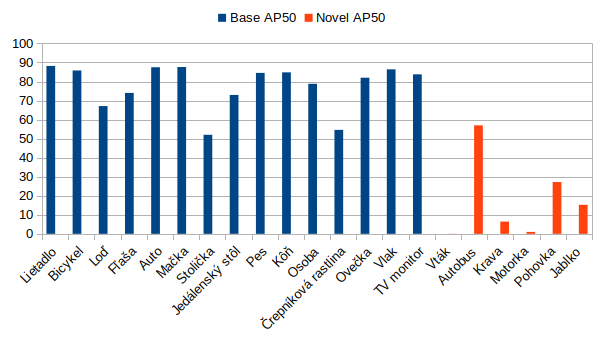
\includegraphics[width=\textwidth]{images/1_shot_classes_AP50.png}
\centering
\caption{AP50 pre jednotlivé triedy}
\label{fig:image18}
\end{figure}

\begin{figure}[H]
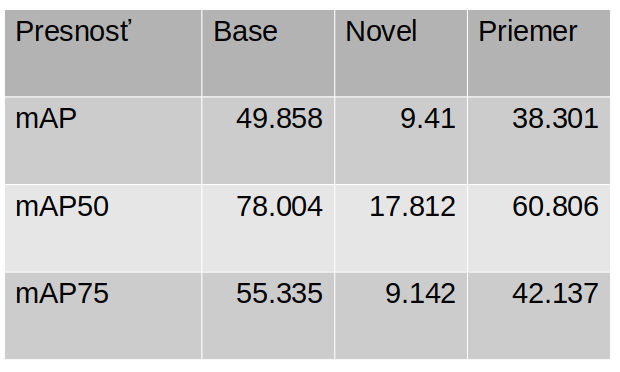
\includegraphics[width=\textwidth]{images/1shot_table_meanAP.png}
\centering
\caption{Tabuľka presnosti pre všetky triedy}
\label{fig:image19}
\end{figure}

\begin{figure}[H]
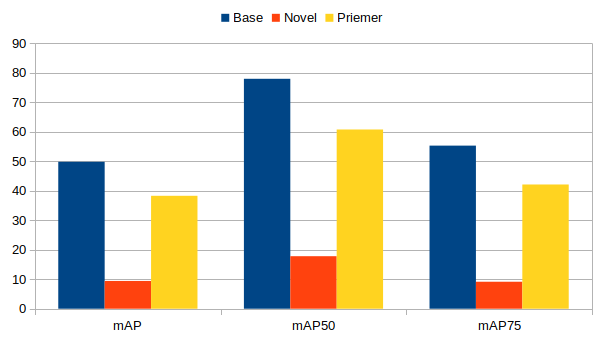
\includegraphics[width=\textwidth]{images/1_shot_meanAP.png}
\centering
\caption{Celková presnosť pre všetky triedy}
\label{fig:image20}
\end{figure}


\subsubsection{2-shot detekcia}

\begin{figure}[H]
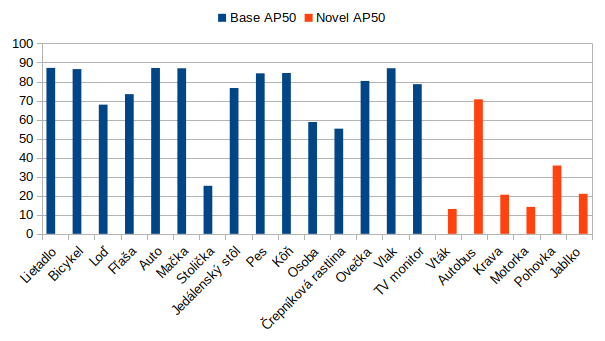
\includegraphics[width=\textwidth]{images/2_shot_classes_AP50.png}
\centering
\caption{AP50 pre jednotlivé triedy}
\label{fig:image21}
\end{figure}

\begin{figure}[H]
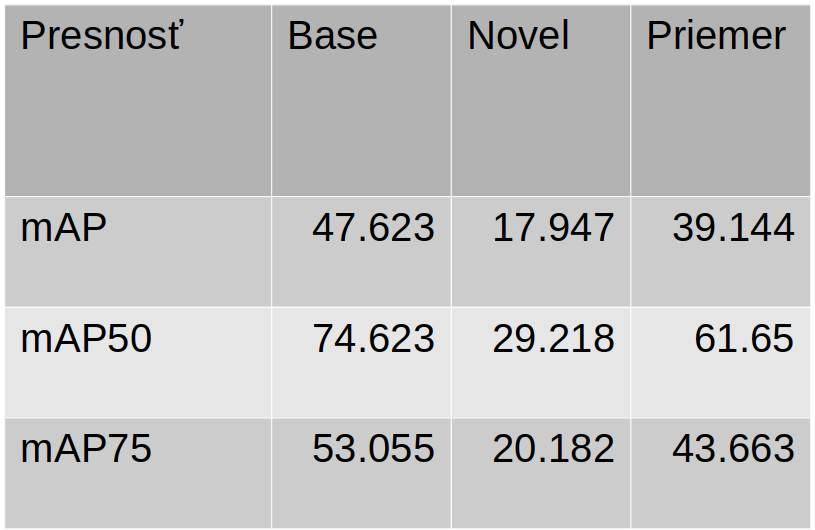
\includegraphics[width=\textwidth]{images/2shot_table_meanAP.png}
\centering
\caption{Tabuľka presnosti pre všetky triedy}
\label{fig:image22}
\end{figure}

\begin{figure}[H]
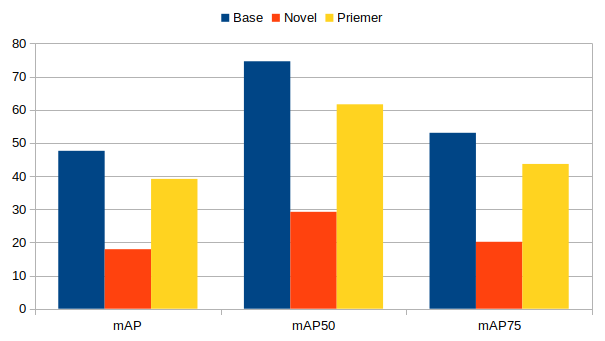
\includegraphics[width=\textwidth]{images/2_shot_meanAP.png}
\centering
\caption{Celková presnosť pre všetky triedy}
\label{fig:image23}
\end{figure}

Celkový čas tréningu: 1 hodina, 51 minút a 41 sekúnd, na obrázku \ref{fig:image21} vidíme presnosť AP50 pre jednotlivé triedy, vidíme, že rozloženie presnosti sa zlepšila oproti 1-shot detekcii a už dokážeme rozpoznať každý objekt aspoň s nejakou presnosťou. Na obrázku \ref{fig:image22} a \ref{fig:image23} vidíme priemernú presnosť nášho modelu.

\subsubsection{3-shot detekcia}

\begin{figure}[H]
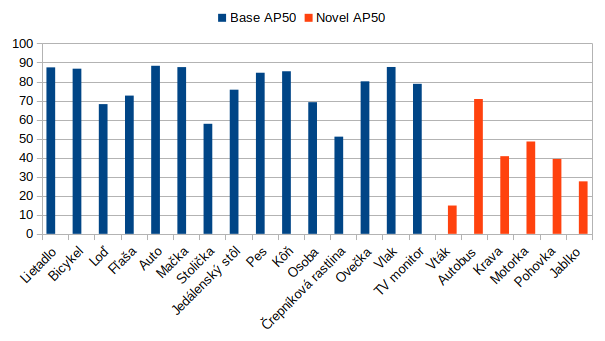
\includegraphics[width=\textwidth]{images/3_shot_classes_AP50.png}
\centering
\caption{AP50 pre jednotlivé triedy}
\label{fig:image25}
\end{figure}

\begin{figure}[H]
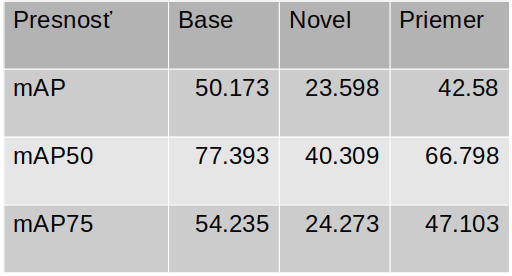
\includegraphics[width=\textwidth]{images/3shot_table_meanAP.png}
\centering
\caption{Tabuľka presnosti pre všetky triedy}
\label{fig:image26}
\end{figure}

\begin{figure}[H]
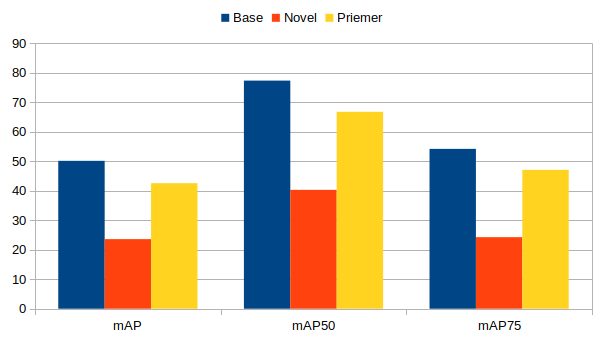
\includegraphics[width=\textwidth]{images/3_shot_meanAP.png}
\centering
\caption{Celková presnosť pre všetky triedy}
\label{fig:image27}
\end{figure}

Celkový čas tréningu: 2 hodiny, 46 minút a 44 sekúnd, na obrázku \ref{fig:image25} vidíme presnosť AP50 pre jednotlivé triedy, vidíme, že rozloženie presnosti sa opäť zlepšilo, ale pre triedu vták je stále dosť nízka presnosť. Na obrázku \ref{fig:image26} a \ref{fig:image27} vidíme priemernú presnosť nášho modelu.

\subsubsection{5-shot detekcia}

\begin{figure}[H]
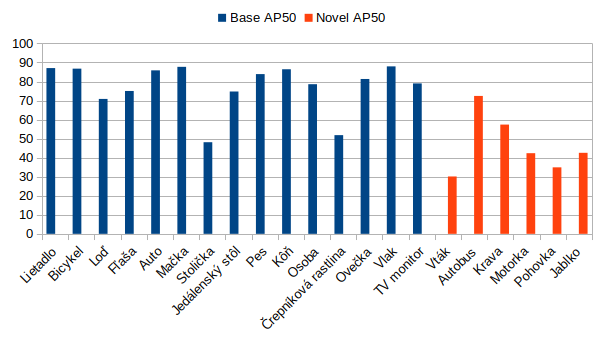
\includegraphics[width=\textwidth]{images/5_shot_classes_AP50.png}
\centering
\caption{AP50 pre jednotlivé triedy}
\label{fig:image28}
\end{figure}

\begin{figure}[H]
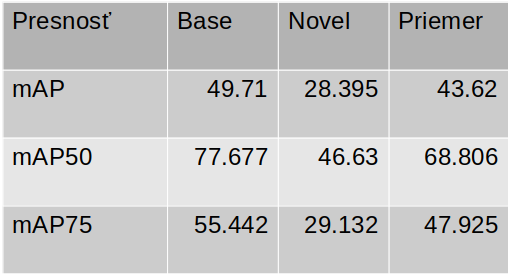
\includegraphics[width=\textwidth]{images/5shot_table_meanAP.png}
\centering
\caption{Tabuľka presnosti pre všetky triedy}
\label{fig:image29}
\end{figure}

\begin{figure}[H]
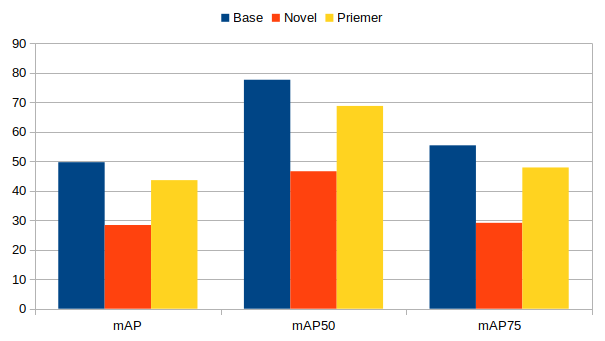
\includegraphics[width=\textwidth]{images/5_shot_meanAP.png}
\centering
\caption{Celková presnosť pre všetky triedy}
\label{fig:image30}
\end{figure}

Celkový čas tréningu: 4 hodiny, 35 minút a 25 sekúnd. Ako vidíme tréningový čas nám veľmi rastie pri zvyšovaní počtu trénovacích obrázkov, keďže taktiež treba zvyšovať počet iterácií, aby sme dosiahli optimálne výsledky. Na obrázku \ref{fig:image28} vidíme presnosť AP50 pre jednotlivé triedy, vidíme, že rozloženie presnosti sa zvyšovaním počtu trénovacích obrázkov stále zvyšuje a tentokrát už máme pre každú triedu AP50 nad 30. Na obrázku \ref{fig:image29} a \ref{fig:image30} vidíme priemernú presnosť nášho modelu.

\subsubsection{10-shot detekcia}

\begin{figure}[H]
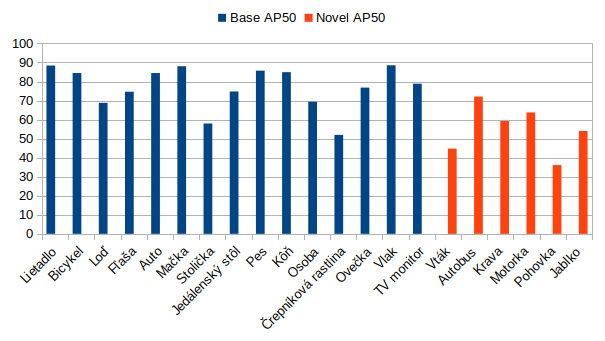
\includegraphics[width=\textwidth]{images/10_shot_classes_AP50.png}
\centering
\caption{AP50 pre jednotlivé triedy}
\label{fig:image31}
\end{figure}

\begin{figure}[H]
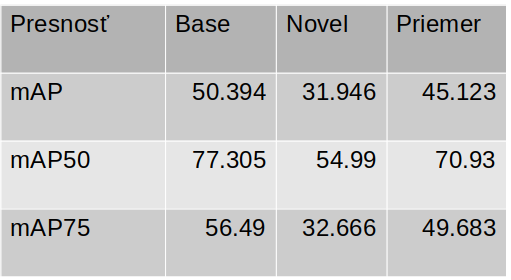
\includegraphics[width=\textwidth]{images/10shot_table_meanAP.png}
\centering
\caption{Tabuľka presnosti pre všetky triedy}
\label{fig:image32}
\end{figure}

\begin{figure}[H]
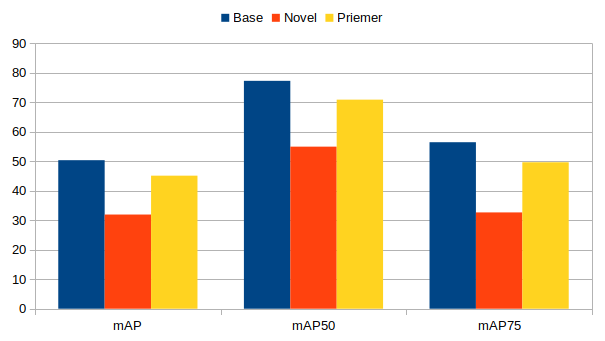
\includegraphics[width=\textwidth]{images/10_shot_meanAP.png}
\centering
\caption{Celková presnosť pre všetky triedy}
\label{fig:image33}
\end{figure}

Celkový čas tréningu: 9 hodín, 11 minút a 4 sekundy. Na obrázku \ref{fig:image31} vidíme presnosť AP50 pre jednotlivé triedy. Na obrázku \ref{fig:image32} a \ref{fig:image33} vidíme priemernú presnosť nášho modelu.

\subsubsection{15-shot detekcia}

\begin{figure}[H]
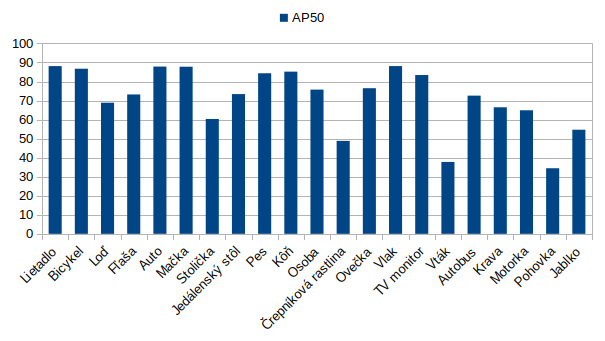
\includegraphics[width=\textwidth]{images/15_shot_classes_AP50.png}
\centering
\caption{AP50 pre jednotlivé triedy}
\label{fig:image34}
\end{figure}

\begin{figure}[H]
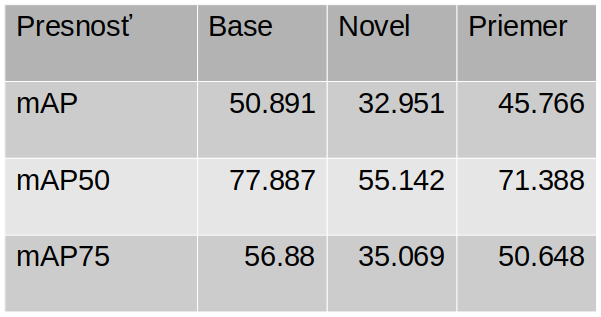
\includegraphics[width=\textwidth]{images/15shot_table_meanAP.png}
\centering
\caption{Tabuľka presnosti pre všetky triedy}
\label{fig:image35}
\end{figure}

\begin{figure}[H]
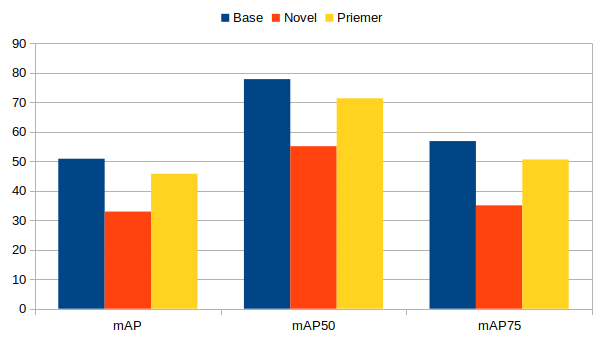
\includegraphics[width=\textwidth]{images/15_shot_meanAP.png}
\centering
\caption{Celková presnosť pre všetky triedy}
\label{fig:image36}
\end{figure}

Celkový čas tréningu: 13 hodín, 56 minút a 37 sekúnd. Na obrázku \ref{fig:image34} vidíme presnosť AP50 pre jednotlivé triedy. Na obrázku \ref{fig:image35} a \ref{fig:image23} vidíme priemernú presnosť nášho modelu. Presnosť nášho modelu sa len minimálne zvýšila oproti 10-shot detekcii a pritom dĺžka tréningu sa zvýšila približne o 50 percent.

\subsection{Vyhodnotenie}

Terazvyhodnotíme rôzne vlastnosti fine-tuningu vzhľadom k počtu trénovacích obrázkov. 

\begin{figure}[H]
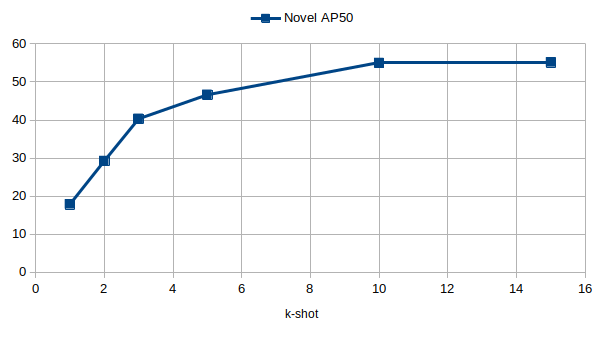
\includegraphics[width=\textwidth]{images/results_novel_AP50.png}
\centering
\caption{Novel AP50 vzhľadom k počtu trénovacích obrázkov}
\label{fig:image37}
\end{figure}

Na obrázku \ref{fig:image37} vidíme presnosť novel tried vzhľadom k počtu trénovacíh obrázkov. Vidíme, že presnosť nám stále stúpa, ale po 10tich trénovacích obrázkoch nám presnosť stúpa už iba minimálne. Pri pätnástich trénovacích obrázkoch nám oproti desiatim stúpla presnosť iba o zanedbatelných 0.153.

\begin{figure}[H]
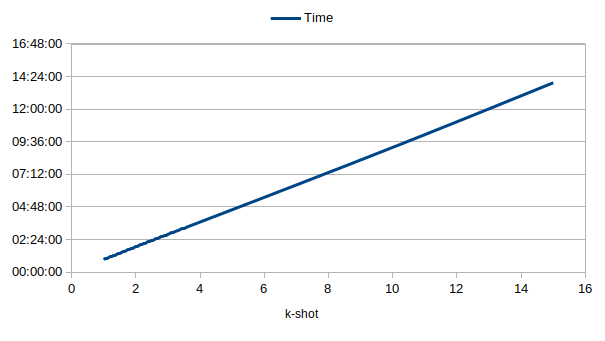
\includegraphics[width=\textwidth]{images/results_time.png}
\centering
\caption{Čas tréningu vzľadom k počtu trénovacích obrázkov}
\label{fig:image38}
\end{figure}

Na ďaľšom obrázku \ref{fig:image38} vidíme ako sa nám mení čas tréningu, vzhľadom k počtu trénovacích obrázkov. Vidíme lineárnu funkciu, čas tréningu nám priamoúmerne stúpa s počtom trénovacích obrázkov.

\begin{figure}[H]
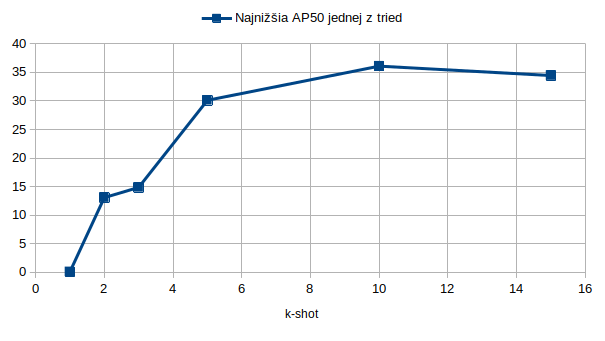
\includegraphics[width=\textwidth]{images/results_lowest_AP50.png}
\centering
\caption{Najnižia AP50 vzhľadom k počtu trénovacích obrázkov}
\label{fig:image39}
\end{figure}

Ďalšia zaujímava metrika na obrázku \ref{fig:image39} nám ukazuje presnosť tierdy s najmenšou presnosťou vzhľadom k počtu trénovacích obrázkov. Vidíme, že pri 1-shot detekcii jedna z tried má takmer nulovú presnosť, čo nie je úplne ideálne, keď je pre nás dôležité rozpoznávať všetky triedy. Tento graf nám teda zobrazuje garanciu najnižej presnosti pre každú z tried bez ohľadu na priemernú prenosť. Vidíme, že od 5-shot learningu máme celkom solidnú garanciu aspon 30 percent AP50 pre každú triedu. Pri 15-shot detekcii sa nám najnižia presnosť dokonca o trochu zníži oproti 10-shot detekcii, napriek jemnému zvýšeniu priemernej presnosti. 






